\documentclass[8.01x]{subfiles}
\begin{document}

\chapter{Midterm 2}

\section{Problem 1: Gravitational potential, kinetic energy, conservation of mechanical energy}

``A meteorite of mass $m = \SI{2e4}{kg}$ is approaching head-on a planet of mass $M = \SI{7e29}{kg}$ and radius $R = \SI{3e4}{km}$. Assume that the meteorite is initially at a very large distance from the planet where it has a speed $v_0 = \SI{4e2}{km/s}$. Take $G = \num{6.67e-11}$.

Determine the speed of the meteorite $v$ (in m/s) just before it hits the surface of the planet. (The planet has no atmosphere, so we can neglect all friction before impact)''

Because the two start out separated by a ``very large distance'', I assume that $U_{initial} = 0$ (that is, we treat the separation as infinitely large). If we find gravitational potential energy at the planet's surface, and then calculate the change in potential energy, we can apply the conservation of mechanical energy to find the meteorite's kinetic energy, and from that, the impact speed.\\
In doing so, we assume that the planet's movement and change in kinetic energy is negligible.

Initial kinetic energy is $\displaystyle \frac{1}{2} m v_0^2$, while initial potential energy is zero.\\
The final kinetic energy is $\displaystyle \frac{1}{2} m v^2$ where $v$ is the impact velocity; final potential energy is $\displaystyle - \frac{G M m}{R}$. Note that the final potential energy is \emph{negative}, and therefore \emph{smaller} than the initial, despite the initial being zero.

Conservation of mechanical energy gives us $K + U = K' + U'$, using the prime notation to mean ``after'' (or at the collision, rather), so we get

\begin{align}
\frac{1}{2} m v_0^2 + 0 &= \frac{1}{2} m v^2 + \left( - \frac{G M m}{R} \right)\\
m v_0^2 + \frac{2 G M m}{R} &= m v^2
\end{align}
\begin{equation}
v = \sqrt{v_0^2 + \frac{2 G M}{R}} \approx \SI{1.809e6}{m/s}
\end{equation}

Since this is an exam, and since 1800 km/s is a very high speed, let's just ensure that the total energy didn't change.\\
Initial kinetic energy of the meteorite was $\SI{1.6e15}{J}$ (holy smokes), which equals the initial energy.\\
Final kinetic energy is $\SI{3.27e16}{J}$, while final potential energy is $\SI{-3.11e16}{J}$, so the final energy total is $\SI{1.6e15}{J}$.\\
Excellent.

\section{Problem 2: Cylinder on turntable}

\begin{center}
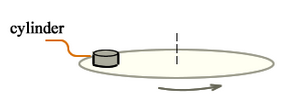
\includegraphics[scale=0.8]{Graphics/midterm2p2}
\end{center}

``Suppose the metal cylinder shown above has a mass of $m = \SI{0.10}{kg}$ and that the coefficient of static friction between the surface and the cylinder is $\mu = 0.12$. If the cylinder is $x = 0.20$ m from the center of the turntable, what is the maximum speed $v_{max}$ that the cylinder can move along its circular path without slipping off the turntable? Choose the range that includes your answer.''

There needs to be a centripetal force on the cylinder for it to stay where it is. This force is provided by the contact force between the cylinder and the surface; friction, in other words. The force required is $\displaystyle \frac{m v^2}{x}$. The maximum possible frictional force is given by $\mu m g$. No other forces are relevant, so the condition is

\begin{align}
\frac{m v_{max}^2}{x} = \mu m g\\
v_{max} = \sqrt{x \mu g}
\end{align}

The equation is dimensionally consistent, and it says that $v_{max} = \SI{0.4898}{m/s}$ using $g = \SI{10}{m/s^2}$, or very slightly less using $g = \SI{9.81}{m/s^2}$.

In either case, the answer is in the range $0.0 < v_{max} \le 0.5$ m/s, so that's the answer.

\section{Problem 3: Woman in elevator}

``A woman weighs $F_g = \SI{550}{N}$ when standing on a stationary scale. Now, the woman is riding an elevator from the 1st floor to the 10th floor. As the elevator approaches the 10th floor, it decreases its upward speed from 6 m/s to 1 m/s in a time interval of 2 seconds. What is the average force exerted by the elevator floor on this woman during this 2 s interval? Use $g = \SI{10}{m/s^2}$.''

This shouldn't be too hard. With only one attempt however, since it is multiple choice, I still saved this (and problem 2) for last.

As the speed decreases, her momentum changes from $(\SI{55}{kg})(\SI{6}{m/s}) = 330$ kg m/s to $(\SI{55}{kg})(\SI{1}{m/s}) = 55$ kg m/s. That's an impulse of $I = p_f - p_i = -275$ kg m/s.\\
(Her mass is $\displaystyle \frac{F_g}{g} = \frac{\SI{550}{N}}{\SI{10}{m/s^2}} = \SI{55}{kg}$.)

The impulse can be used to find the average force (not the final answer, mind you, we still need to consider $m g$):

\begin{align}
\Braket{F} (\SI{2}{s}) = \SI{-275}{kg m/s}\\
\Braket{F} = \frac{\SI{-275}{kg m/s}}{\SI{2}{s}} = \SI{-137.5}{N}
\end{align}

She is then 137.5 N lighter than usual as the elevator slows down. Her net weight is $\SI{550}{N} + \SI{-137.5}{N} = \SI{412.5}{N}$. This is the same as the force the floor exerts on her (the force the floor exerts on you \emph{is} your weight, according to our definitions).

A second way of solving this is to consider acceleration. When the elevator is slowing down, the perceived gravity decreases. The elevator's average acceleration is

\begin{equation}
a_{avg} = \frac{\SI{1}{m/s} - \SI{6}{m/s}}{\SI{2}{s}} = \SI{-2.5}{m/s^2}
\end{equation}

The perceived gravity is then $g + (\SI{-2.5}{m/s^2}) = \SI{7.5}{m/s^2}$, and her weight is $m g = 412.5$ N.

\section{Problem 4: Two skaters}

``Two skaters of mass $m_1 = \SI{50}{kg}$ and $m_2 = \SI{70}{kg}$ are standing motionless on a horizontal ice surface. They are initially a distance $L = 8.0$ meters apart. They hold a massless rope between them. After pulling the rope, the skater of mass $m_1$ has moved a distance $\ell = 1.0$ meters away from his initial position. We can completely neglect friction in this problem.

What is the distance $L'$ between the two skaters when the skater of mass $m_1$ has moved a distance $\ell$? (in meters)''

Oh. I read the problem at least three times before realizing that \emph{both} skaters will move... Silly me.

Okay, so what do we know? With no external forces (such as friction) in the horizontal direction, conservation of momentum holds. Not knowing any final velocity, this might seem to be of limited usefulness, but let's see!\\
Since the initial velocities are both zero, I will use $v_1$ and $v_2$ for the velocities they move at after the fact. Initial momentum is zero and is conserved, so

\begin{equation}
m_1 v_1 + m_2 v_2 = 0
\end{equation}

From that, we can find

\begin{equation}
\frac{v_1}{v_2} = - \frac{m_2}{m_1}
\end{equation}

\begin{equation}
v_2 = - \frac{m_1 v_1}{m_2}
\end{equation}

$v_1$ moved a distance $\ell$ under some unknown time $t$; what distance did $v_2$ move under that same time? He moved a distance $m_1/m_2$ times as great (the ratio of their speeds), and clearly they both went towards each other.

They came $\ell = 1.0$ meters closer due to the movement of $m_1$, and $\displaystyle \frac{m_1}{m_2} \ell = 5/7$ meters closer due to the moment of $m_2$. Therefore,

\begin{equation}
L' = L - \ell \left(1  + \frac{m_1}{m_2}\right) \approx \SI{6.286}{m}
\end{equation}

\section{Problem 5: Sliding down a dome}

\begin{center}
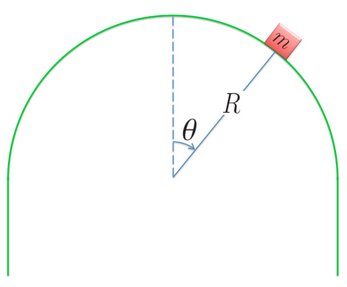
\includegraphics[scale=0.8]{Graphics/midterm2p5}
\end{center}

``A small object of mass $m = \SI{20}{kg}$ slides down a spherical dome of radius $R = \SI{12}{m}$ without any friction. It starts off at the top (polar angle $\theta = 0$) at zero speed. Use $g = \SI{10}{m/s^2}$. (See figure)

(a) What is the magnitude of the force (in Newtons) exerted by the dome on the mass when it is at the top, at $\theta = \ang{0}$?\\
(b) What is the magnitude of the force (in Newtons) exerted by the dome on the mass when it is at $\theta = \ang{30}$?\\
(c) At what angle $\theta_0$ does the sliding mass take off from the dome? Answer in degrees ($0 \le \theta_0 \le \ang{90}$).''

Hmm, I assume this problem is meant to be similar to one previously, which stated that it started with a negligible but nonzero speed. It should be in a stable equilibrium at the top, so with exactly zero speed, it should stay there forever!

At $\theta = 0$, the normal force should be simply $m g = 200$ N. It is at rest, there are no forces other than gravity and the normal force, and the two must balance out exactly or it wouldn't be at rest.

What is the normal force for other values of $\theta$, though? At 90 degrees, it's clearly zero, as there's nothing to make it stick to the dome, and no reason for the two to still be in contact at that point. However, it becomes zero earlier: when the object loses contact with the surface (question c).

When does it ``take off'', though? How can we find a simple criterion to calculate at which angle that happens?\\
Well, for it to move in along this circular (in cross section, at least) dome, it needs to have a certain centripetal force inwards.

The criterion for falling off is then that the centripetal force is no longer strong enough to keep the tangential velocity changing along a circular path. The centripetal force required is $\displaystyle \frac{m v^2}{R}$.\\
The forces that can provide this force is gravity and the normal force. In decomposing the force of gravity, we find $m g \cos \theta$ in the radially inwards direction (perpendicular to the surface) and $m g \sin \theta$ in the tangential direction; we only need the radial part here, though.

The centripetal force is always radially inwards; the radial component of gravity $m g \cos \theta$ is also inwards, but the normal force is radially \emph{outwards}, and so contributes a minus sign:

\begin{equation}
\frac{m v^2}{R} = m g \cos \theta - N
\end{equation}
\begin{equation}
N = m g \cos \theta - \frac{m v^2}{R}
\end{equation}

When the object falls off, $N$ must be zero (there can't be any contact forces without contact!). That gives us the condition

\begin{align}
g \cos \theta_0 &= \frac{v_{off}^2}{R}\\
\theta_0 &= \arccos \frac{v_{off}^2}{g R} \label{midterm2:t0}
\end{align}

(I call the speed $v_{off}$ specifically because I accidentally used it as a general value for part (b), which gave me the wrong answer. I thankfully figured that out before submitting, but it took a while to realize my mistake!)

Unfortunately, we don't know $v_{off}$! We can find the tangential acceleration, but since there are only conservative forces involved, mechanical energy is conserved, so we can use an energy approach and forget about the kinematics.

Say we define $U = 0$ at the point where $\theta = \ang{90}$. That means the initial gravitational potential energy is $m g R$; what about the final energy? It is not zero, since the object will fly off prior to reaching the zero point.\\
We can find the height above the zero point in terms of $\theta_0$. Drawing it out, some trigonometry shows that $h = R \cos \theta_0$. This is consistent with $h$ being a maximum at $\theta = 0$ and zero at $\theta = \ang{90}$, which is always a good sign!

The gain in kinetic energy must equal the loss in potential energy. Since the kinetic energy started out at zero, we find:

\begin{equation}
\frac{1}{2} m v_{off}^2 = m g R - m g R \cos \theta
\end{equation}

However, we have an expression for $\theta_0$ in equation \eqref{midterm2:t0} which is the only angle of  $\theta$ we care about for part (c); taking the cosine of both sides gives us $\displaystyle \cos \theta_0 = \frac{v_{off}^2}{g R}$, so we substitute that in the velocity equation above:

\begin{align}
\frac{1}{2} m v_{off}^2 &= m g R - m v_{off}^2\\
v_{off}^2 &= 2 g R - 2v_{off}^2\\
v_{off} &= \sqrt{\frac{2 g R}{3}}
\end{align}

This is then the speed it has as it falls off. 

We can then use this value for $\theta_0$:

\begin{align}
\theta_0 &= \arccos \frac{\frac{2 g R}{3}}{g R}\\
\theta_0 &= \arccos \frac{2}{3} \approx \ang{48.1897}
\end{align}

Incredibly, $g$, $R$ and $m$ all cancel at some point, and the angle is a constant! Honestly, this is a bit mind-blowing to me. I would at least expect $g$ to matter, but nope.

We can find a general value of $v$, which is valid for all angles, by going back to the conservation of energy equation:

\begin{align}
\frac{1}{2} m v^2 &= m g R - m g R \cos \theta\\
v^2 &= 2 g R (1- \cos \theta)\\
v &= \sqrt{2 g R (1- \cos \theta)}
\end{align}

We need that to find the normal force at 30 degrees. We found an expression for that earlier, but now we also know $v$, so we can find $N$ in terms of only known values:

\begin{align}
N &= m g \cos \theta - \frac{m v^2}{R}\\
N &= m g \cos \theta - \frac{2 m g R (1 - \cos \theta)}{R}\\
N &= m g (\cos \theta - 2 (1 - \cos \theta))\\
N &= m g (3\cos \theta - 2) \approx \SI{119.615}{N}
\end{align}

So the answers are

(a) Normal force at $\theta = 0$: $m g = 200$ N\\
(b) Normal force at $\theta = \ang{30}$: $119.615$ N\\
(c) Angle where it slides off: $\theta_0 = \ang{48.1897}$

\section{Problem 6: Pendulum with cut string}

A small ball of mass $m = 0.60$ kg hangs from a massless string of length $\ell = 1.4$ m. The ball travels in a vertical circle and its speed at the bottom is $v_0 = 7.0$ m/s (see figure). Neglect all friction and air drag, and use $g = \SI{10}{m/s^2}$ for the gravitational acceleration. The ball is so small that we can approximate it as a point.

\begin{center}
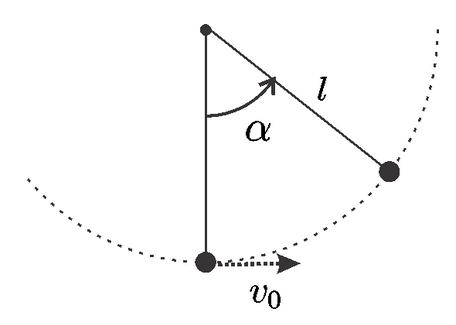
\includegraphics[scale=0.5]{Graphics/midterm2p6}
\end{center}

(a) Find the speed of the ball (in m/s) when the string is at $\alpha = \ang{50}$.\\
(b) What is the tension in the string (in Newton) when it is at $\alpha = \ang{50}$?\\
(c) The string of the pendulum is cut when it is at $\alpha = \ang{50}$. First, we want to neglect all air drag during the trajectory of the ball.\\
What is the maximal height $h$ (in meters) the ball reaches above its point of release?\\
What time $t_{up}$ (in s) does it take the ball to reach the highest point from the instant the string is cut?\\
What time $t_{dn}$ (in s) does it take the ball to go from the highest point back to the altitude it was released from the string?

(d) Next, we want to take air drag into account for point (c). Let $\widetilde{h}$ be the maximal height of the ball above the point it was released, $\widetilde{t_{up}}$ is the time to get there, and $\widetilde{t_{dn}}$ is the time to get back to the altitude it was released (with air drag). Which of the following is true? (neglect the effect of air drag before the string is cut)

(d1)

\begin{itemize}
\item $\widetilde{h}$ is always greater than $h$
\item $\widetilde{h}$ is always smaller than $h$
\item $\widetilde{h}$ is the same as $h$
\item We need to know if the ball is is the pressure dominated regime or in the viscous regime to tell whether $\widetilde{h} > h$, $\widetilde{h} < h$ or $\widetilde{h} = h$.
\end{itemize}

(d2)
\begin{itemize}
\item $\widetilde{t_{up}} > \widetilde{t_{dn}}$ and $\widetilde{t_{dn}} < t_{dn}$
\item $\widetilde{t_{up}} < \widetilde{t_{dn}}$ and $\widetilde{t_{up}} < t_{up}$
\item $\widetilde{t_{up}} = \widetilde{t_{dn}}$ and $\widetilde{t_{up}} < t_{up}$
\item $\widetilde{t_{up}} > \widetilde{t_{dn}}$ and $\widetilde{t_{up}} > t_{up}$
\item The answer depends on whether the initial speed is larger or smaller than the terminal speed.
\end{itemize}

WOW! That took a while to typeset properly (copy/paste doesn't work for the math notation, unfortunately)!

Okay, so let's start. The string tension is perpendicular to the ball's movement at all times, and therefore cannot do work. This means that gravity is the only force that \emph{can} do work. Because of that, 100\% of the loss in kinetic energy is converted to gravitational potential energy.\\
We can use conservation of energy, considering only kinetic energy and gravitational potential energy.

We define the zero point of potential energy to be at $\alpha = 0$, for simplicity. We can then calculate the potential energy at $\alpha = \ang{50}$, relate the initial and final total energies: $K + U = K' + U'$, using prime notation for the ``after'' energies (at $\alpha = \ang{50}$).

First, however, we need to find a way to calculate the height above the zero point (I'll call it $h$) in terms of $\ell$ and $\alpha$.\\
Drawing it out, it can be seen that $h = \ell - \ell \cos \alpha = \ell (1 - \cos \alpha)$ (in a way identical to what was done for the pendulum in lecture).

Knowing that, we can now relate the initial energy (left-hand side) and final energy (right-hand side) as the string is cut:

\begin{align}
\frac{1}{2} m v_0^2 + 0 &= \frac{1}{2} m v^2 + m g \ell (1 - \cos \alpha)\\
v_0^2 &= v^2 + 2 g \ell (1 - \cos \alpha)\\
v^2 &= v_0^2 - 2 g \ell (1 - \cos \alpha)\\
v &= \sqrt{v_0^2 - 2 g \ell (1 - \cos \alpha)}
\end{align}

We can then answer part (a). With the numbers given, $v(\alpha = \ang{50}) = \SI{6.2448}{m/s}$.

Next, they want to know the tension at this point. We can find it by relating all the forces in the radial direction. The tension is always perpendicular to the pendulum's movement, so there is no tension in the tangential direction.

In order to move along the circular path, there needs to be a centripetal force $\displaystyle m a_c = \frac{m v^2}{\ell}$ radially inwards. Gravity and tension are the two forces that can help provide this.\\
We first need to decompose the gravitational force, since we only want the radial component. The radial component is $m g \cos \theta$ in magnitude, and is radially outwards at $\theta = 0$. Newton's second law in the radially inwards direction gives us

\begin{align}
\frac{m v^2}{\ell} &= T - m g \cos \alpha\\
T &= \frac{m v^2}{\ell} + m g \cos \alpha\\
T &= \frac{m}{\ell}\left( v_0^2 - 2 g \ell (1 - \cos \alpha) \right) + m g \cos \alpha\\
T &= \frac{m}{\ell} v_0^2 - 2 g m (1 - \cos \alpha) + m g \cos \alpha\\
T &= \frac{m}{\ell} v_0^2 - m g (2 - 3\cos \alpha)
\end{align}

This gives us a tension, at $\alpha = \ang{50}$, of \SI{20.57}{N}.\\
The equation also makes intuitive sense: higher $v_0$ means higher tension, and there are $v_0$-$\alpha$ combinations where $v_0$ is not great enough for the tension to be positive -- that is, if $v_0$ is too small, it will never reach that angle.

Now, then, on to the interesting stuff. The string is cut at the above point. What the the height $h$ it reaches, measured \emph{above the point of release}, if we neglect air drag?

Okay, so we can use an energy based approach here, too, since we neglect air drag. I will re-use the variable name $h$, and re-define $U = 0$ to be at the height it is now, and call that height zero as well. We know $v$, so we can easily find the kinetic energy. Again, gravity is the only force that will reduce the kinetic energy, and so the entire reduction in kinetic energy will be converted into gravitational potential energy. Initial kinetic energy depends on $v$, but final kinetic energy on $v \cos \theta$. The $y$ component, $v \sin \theta$, will have gone down to zero, while the $x$ component remains untouched. Using conservation of energy (and keep in mind that this $h$ is unrelated to everything prior to this):

\begin{align}
\frac{1}{2} m v^2 + 0 &= \frac{1}{2} m (v \cos \alpha)^2 + m g h\\
m v^2 + 0 &= m v^2 \cos^2 \alpha + 2 m g h\\
\frac{v^2 (1 - \cos^2 \alpha)}{2 g} &= h\\
\frac{v^2 \sin^2 \alpha}{2 g} &= h
\end{align}

This gives us a height of $h = 1.1442$ m. It doesn't give us the time, though... Should've thought of that.\\
We can find the same result using kinematics, by finding the time where the velocity becomes 0. We can then substitute that time into the displacement equation $\displaystyle h = x_0 + v t_{up} + \frac{1}{2} a t_{up}^2$ to find the height that way, too:

However, we must keep in mind that the upwards velocity is not $v$, but $v \sin \alpha$.

\begin{align}
v \sin \alpha - g t_{up} = 0 &\Rightarrow t_{up} = \frac{v \sin \alpha}{g}\\
h = v \sin \alpha t_{up} - \frac{1}{2} g t_{up}^2 &\Rightarrow h = \frac{v^2 \sin^2 \alpha}{2 g}
\end{align}

We find the same height, but also the time taken: the upwards velocity, divided by $g$, a familiar result. In terms of numbers, $t_{up} = 0.47838$ seconds.\\
And after that, the time for the ball to fall back down. Without air drag, this is a symmetric problem, so the time must be the same. Let's verify via kinematics just to be sure:

\begin{align}
h - \frac{1}{2} g t_{dn}^2 &= 0\\
\frac{1}{2} g t_{dn}^2 &= h
\end{align}
\begin{equation}
t_{dn} = \sqrt{\frac{2 h}{g}} \approx \SI{0.47838}{s}
\end{equation}

Finally, the scary-looking part. Without quantitative answers, it shouldn't be that bad, though.
First out:

\begin{itemize}
\item $\widetilde{h}$ is always greater than $h$
\item $\widetilde{h}$ is always smaller than $h$
\item $\widetilde{h}$ is the same as $h$
\item We need to know if the ball is is the pressure dominated regime or in the viscous regime to tell whether $\widetilde{h} > h$, $\widetilde{h} < h$ or $\widetilde{h} = h$.
\end{itemize}

Well, what will happen with air drag? Since they ask us to neglect air drag before the string is cut, the previous results are all valid. All we need to do is compare the trajectory with and without drag.

With drag, there will be a resistive force opposing the motion (relative to the  air), which means a downwards force, and a ``backwards'' force (to the left, as the figure shows the problem). This clearly means it cannot go as high as it would otherwise (the downwards force, and so the downwards acceleration, is greater), so $\widetilde{h}$ must always be smaller than $h$.\\
This is equally true in both regimes (though in air, we are clearly pressure dominated). In both regimes, the force opposes the motion, and so in either, the result will be a lower maximum height.

Next, part 2:

\begin{enumerate}
\item $\widetilde{t_{up}} > \widetilde{t_{dn}}$ and $\widetilde{t_{dn}} < t_{dn}$
\item $\widetilde{t_{up}} < \widetilde{t_{dn}}$ and $\widetilde{t_{up}} < t_{up}$
\item $\widetilde{t_{up}} = \widetilde{t_{dn}}$ and $\widetilde{t_{up}} < t_{up}$
\item $\widetilde{t_{up}} > \widetilde{t_{dn}}$ and $\widetilde{t_{up}} > t_{up}$
\item The answer depends on whether the initial speed is larger or smaller than the terminal speed.
\end{enumerate}

Okay, let's try to rule out some of these.\\
Number 3, $\widetilde{t_{up}} = \widetilde{t_{dn}}$ is not true. With air resistance, a projectile launched with an initial upwards takes \emph{longer} to fall back down, than to come up in the first place. This makes number number 1 and 4 false, too.

Left are number 2 and number 5. Let's tackle them one by one.\\
$\widetilde{t_{up}} < \widetilde{t_{dn}}$ is true, as we have seen. Is $\widetilde{t_{up}} < t_{up}$ also true? If so, this must be the answer.\\
With air drag, it doesn't reach as high, so it makes sense that it takes less time with air drag.\\
On the other hand, with air drag, the speed is constantly lowered by the drag (plus gravity, in either case), which means it takes longer time to reach a certain height... But there's a simple way to show that the the time taken to reach the maximum height must be \emph{less} with air drag acting.

The initial velocity upwards is the same; the time we're looking for is when the net acceleration (or deceleration, if you prefer) has made the upwards velocity 0. With the \emph{same} initial velocity, the case with the greatest downwards force (or acceleration) is clearly the one to stop first, and that is the case \emph{with} air drag. $\widetilde{t_{up}} < t_{up}$ must be the case!

What about option 5? Does the time taken to move upwards depend on whether the initial speed is larger or smaller than the terminal speed? I don't see why it would. That leaves option 2 as the only one possible answer, it looks like! It's always nice to be able to not only find a correct option, but rule out the others, too.

Option 1 is wrong because $\widetilde{t_{up}} < \widetilde{t_{dn}}$, and the option has it the other way around.\\
Option 2 looks good!\\
Option 3 is wrong because $\widetilde{t_{up}} < \widetilde{t_{dn}}$\\
Option 4 is wrong because $\widetilde{t_{up}} < \widetilde{t_{dn}}$\\
Option 5 looks wrong, because the terminal speed has to do with when the drag force (upwards) and gravity (downwards) balance out in a \emph{downwards} fall. There is never any such balance in an upwards motion though air; there will always be deceleration.

These answers are correct, by the way. (I did get $h$, $t_{up}$ and $t_{dn}$ wrong the first time, as I used $v$ instead of $v \sin \alpha$ by accident. D'oh!)

\section{Problem 7: Emergency landing of a plane}

\begin{center}
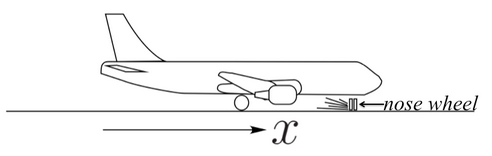
\includegraphics[scale=0.7]{Graphics/midterm2p7}
\end{center}

``An airliner makes an emergency landing with its nose wheel locked in a position perpendicular to its normal rolling position. The forces acting to stop the airliner arise from friction due to the wheels and from the breaking effort of the engines in reverse thrust mode. The force of the engine on the plane is constant, $F_{engine} = -F_0$. The sum of the horizontal forces on the airliner (in its forward direction) can be written as

\begin{equation}
F(t) = - F_0 + \left( \frac{t}{t_s} - 1\right) F_1
\end{equation}

from touchdown at time $t = 0$ to the final stop at time $t_s = 28$ s ($0 \le t \le t_s$).\\
The mass of the plane is $M = 80$ tonnes (one tonne is 1000 kg). We have $F_0 = 260$ kN and $F_1 = 41$ kN. Neglect all air drag and friction forces, except the one stated in the problem.

(a) Find the speed $v_0$ of the plane at touchdown (in m/s).

(b) What is the horizontal acceleration of the plane at the time $t_s$?\\
What is the acceleration at the time of touchdown? (absolute values; in $\text{m/s}^2$)

(c) What distance $s$ does the plane go between touchdown and its final stop at time $t_s$? (in meters)

(d) What work do the engines in reverse thrust mode do during the emergency landing?
(magnitude in Joules; the force due to engines is ($-F_0$))

(e) How much heat energy is absorbed by the wheels during the emergency landing?
(magnitude in Joules; the force due to wheels is $(F(t)+F_0$))''

For part (a), we can use the impulse:

\begin{equation}
\Braket{F} \Delta t = p_f - p_i = -p_i = - M v_0
\end{equation}
\begin{align}
-M v_0 &= \Braket{F} t_s\\
v_0 &= -\frac{\Braket{F} t_s}{M}
\end{align}

The force is linear, so finding the average force should be easy.

\begin{align}
\Braket{F} = \frac{F(0) + F(t_s)}{2} = \frac{-F_0 - F_1 + (- F_0)}{2} = \frac{-2 F_0 - F_1}{2} = \SI{-280500}{N}
\end{align}

We can then find $v_0$:

\begin{align}
v_0 = \frac{(\SI{280500}{N})(\SI{28}{s})}{\SI{80000}{kg}} = \SI{98.175}{m/s}
\end{align}

... or about 353.5 km/h, or 220 mph. We can also find this by realizing that $a = F/M$, and integrating that to find the change in velocity from $t=0$ to $t=t_s$. That yields exactly the above answer.

Next up: acceleration. The only horizontal forces are the forces we're given, so setting up a Newton's second law equation is simple:

\begin{align}
M a &= -F_0 + \left( \frac{t}{t_s} - 1\right) F_1\\
a &= -\frac{F_0}{M} + \left( \frac{t}{t_s} - 1\right) \frac{F_1}{M}
\end{align}

Plugging in numbers,

\begin{align}
a(t=0) &= \SI{-3.7625}{m/s^2}\\
a(t=t_s) &= \SI{-3.25}{m/s^2}
\end{align}

They ask for \emph{magnitudes} though, so we need to get rid of the minus signs.\\
Do the values make sense? Yes, they do. $v_0 - a t_s = 0$, if we use the average of the two as $a$; that is, $a = \SI{-3.50625}{m/s^2}$.

What distance $s$ does the plane move between touchdown and its stop at $t = t_s$?

This is where the problem gets harder. I originally calculated $s$ incorrectly, and then used that to find an incorrect value for part (d) and part (e). $s$ and part (d) \emph{were accepted}, despite being incorrect. The worst part, though, was that part (e) was \emph{not} accepted. The solution was consistent, though -- my answer for (e) was the only one possible if (a) and (d) had been correct, since I related the energies (initial kinetic energy = work by engines + loss to friction). The exact same incorrect answer was found by integrating the work over the distance $s$, since that distance was incorrect!

Let's instead have a look at integrating the acceleration to find the correct answers, which I did for my second try.

If we integrate the acceleration, we find a function for the change in the velocity. $\Delta v$, you might call it.

\begin{align}
\Delta v = \int a \mathop{dt} &= \int \left(-\frac{F_0}{M} + \frac{F_1}{M} \frac{t}{t_s} - \frac{F_1}{M} \right) \mathop{dt}\\
                              &= \int \left(-\frac{F_0 + F_1}{M} + \frac{F_1}{M t_s} t \right) \mathop{dt}\\
                              &= -\frac{t(F_0 + F_1)}{M} + \frac{F_1 t^2}{2 M t_s}
\end{align}

This can be used to find the answer for the initial velocity, as well, by plugging in $t = t_s$ and all numeric values in the above equation. That gives you $\Delta v = -v_0$. The velocity as a function of time is then given by $v(t) = v_0 + \Delta v$:

\begin{equation}
v(t) = v_0 - \frac{t(F_0 + F_1)}{M} + \frac{F_1 t^2}{2 M t_s}
\end{equation}

We can then integrate this over from $t = 0$ to $t = t_s$ to find the distance traveled:

\begin{align}
s &= \int_0^{t_s} \left( v_0 - \frac{t(F_0 + F_1)}{M} + \frac{F_1 t^2}{2 M t_s} \right) \mathop{dt}\\
s &= v_0 t_s + \left[ - \frac{t^2(F_0 + F_1)}{2M} + \frac{F_1 t^3}{6 M t_s} \right]_0^{t_s}\\
s &= v_0 t_s + \left[ - \frac{t_s^2(F_0 + F_1)}{2M} + \frac{F_1 t_s^2}{6 M} \right]
\end{align}

Plugging in the numbers, $s \approx \SI{1340.97}{m}$.

Finding the work by the engines is trivial now: $W_{engines} = -F_0 s = \SI{-348652200}{J}$. They ask for the magnitude, though, so we need to drop the minus sign.

Next, the work done by friction. This is a bit trickier, since we need to integrate in order to solve it by force times distance. Our force is also specified as a function of time, not distance.\\
We can solve it via an energy approach, however.\\
The initial kinetic energy is $\displaystyle \frac{1}{2} M v_0^2$, and the final kinetic energy is exactly zero. Most of the kinetic energy is removed by the engines in reverse thrust, but everything that isn't must be removed as heat by the wheels.

\begin{equation}
|W_{friction}| = \frac{1}{2} M v_0^2 - F_0 s = \SI{385533225}{J} - \SI{348652200}{J} = \SI{36881025}{J}
\end{equation}

\section{Problem 8: Mass pushed by a spring}

``A block of mass $m = 2$ kg on a horizontal surface is connected to a spring connected to a wall (see figure). The spring has a spring constant $k = 14$ N/m. The static friction coefficient between the block and the surface is $\mu_s = 0.5$, and the kinetic friction coefficient is $\mu_k = 0.2$. Use $g = \SI{10}{m/s^2}$ for the gravitational acceleration.

\begin{center}
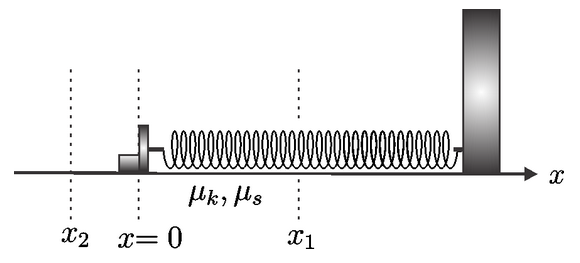
\includegraphics[scale=0.5]{Graphics/midterm2p8}
\end{center}

(a) The spring is initially uncompressed and the block is at position $x = 0$. What is the minimum distance $x_1$ we have to compress the spring for the block to start moving when released? (in meters)

(b) Find the distance $|x_2 - x_1|$ between the point of release $x_1$ found in (a), and the point $x_2$ where the block will come to a stop again. (in meters)

(c) What time $t_{12}$ does it take the block to come to a rest after the release? (i.e., the time of travel between points $x_1$ and $x_2$; in seconds)

(d) What will happen after the block has come to a rest at point $x_2$?

\begin{enumerate}
\item The block will move back towards $x_1$, and it will oscillate with constant frequency and exponentially decreasing amplitude.
\item The block will move back towards $x_1$, and it will oscillate while decreasing both frequency and amplitude.
\item The block will start moving back towards $x_1$, and it will come to a final halt before reaching it.
\item The block will stay at its resting position $x_2$.
\item The answer depends on whether $x_2 > 0$ or $x_2 < 0$.
\end{enumerate}

Hmm, damped oscillations... something which we haven't seen in the course yet, on an exam! I wonder if we can get by withing solving the differential equations, which from what I recall (from similar cases in electronics, from 6.002x) is not easy at all.

At least part (a) should be easy. We need to overcome the maximum possible static friction, $\mu_s N = \mu_s m g$. The spring force is $k x$ in magnitude, so

\begin{align}
k x_1 &> \mu_s m g\\
x_1 &> \frac{\mu_s m g}{k}
\end{align}

For our values, $x_1 > 10/14$ m for the system to not just stay in place.

Okay, so if we release the block at that point (or a micrometer past it), where does the block come to a stop?\\
I would guess that the energy approach is (probably by far) the easiest way to solve this.\\
The spring has potential energy $U = \displaystyle \frac{1}{2} k x_1^2$ stored to begin with.\\
Some of it is turned to kinetic energy, and some of it wasted due to friction.\\
After that, it comes to a halt at $x_2$, at which point there is again energy stored in the spring, $\displaystyle \frac{1}{2} k x_2^2$ this time.

Thankfully, the kinetic friction is constant at $\mu_k N = \mu_k m g$, and so it does work which is simply $-\mu_k m g |x_2 - x_1|$.\\
Adding it all up, energy after and energy before minus losses:

\begin{align}
\frac{1}{2} k x_2^2 &= \frac{1}{2} k x_1^2 - \mu_k m g |x_2 - x_1|\\
\end{align}

In order to get rid of the absolute value signs, we can think for a bit. Will $x_2 > x_1$, always? No, it will move in the opposite direction. $x_1 > x_2$ always, on the other hand. Therefore, we can negate the expression to $x_1 - x_2$ and remove the absolute value signs.

\begin{align}
\frac{1}{2} k x_2^2 &= \frac{1}{2} k x_1^2 - \mu_k m g (x_1 - x_2)\\
k x_2^2 &= k x_1^2 - 2 \mu_k m g (x_1 - x_2)\\
k x_2^2 - 2 \mu_k m g x_2 &= k x_1^2 - 2 \mu_k m g x_1
\end{align}
\begin{equation}
x_2^2 - x_2 \frac{2 \mu_k m g}{k} - x_1^2 + \frac{2 \mu_k m g x_1}{k} = 0
\end{equation}

This is a bit too bad for me to rearrange and solve symbolically, so let's try this:

\begin{equation}
x_2^2 - x_2 (\SI{4/7}{m}) - \SI{10/14}{m} + \SI{20/49}{m} = 0
\end{equation}

\begin{align}
x_2 &= \frac{4}{2\times7} \pm \frac{1}{2} \sqrt{(4/7)^2 - 4 (-5/49)}
\end{align}

This yields two answers: $x_2 = x_1$ which is clearly not the answer we want, and $x_2 = -1/7$.\\
The distance is then $|-1/7 - 10/14| = 0.85714$ m.

Next, they want us to find the amount of time that this movement took. The force follows a single equation the entire journey, so we should be able to solve this.

$+x$ is to the right, so $+m a$ in Newton's second law will be on the left side. On the right, we have the spring force $-k x$ and the friction $F_f = +\mu_k m g$ (which is constant). We can write $a$ as $\ddot{x}$.

\begin{align}
m \ddot{x} &= \mu_k m g - k x\\
\ddot{x} + \frac{k}{m} x  &= \mu_k g
\end{align}

This is a bit familiar. For a vertical oscillator like this, we have a very similar expression. The term $\mu_k g$ turns out to not change the period of the oscillation, but only change the center position and/or amplitude. In other words, we can use the formula for the period we already know (see below for why):

\begin{equation}
T = \frac{2 \pi}{\omega} = 2 \pi \sqrt{\frac{m}{k}}
\end{equation}

However, they don't ask us for the period, but rather the time it takes the block to come to a rest. I would say that's half a period -- from one extreme to the other.
We find $t = 1.18741$ seconds using $\omega_0 / 2$. Can it be trusted?

I also solved the differential equation (with Mathematica), and set set $x_2 = x(t)$ and solved for time, using the values above.\\
The cosine term in the solution to this equation is $\cos \left(\frac{k t}{\sqrt{k m}}\right) = \cos (\omega_t)$. Solving that equation, the end result is then exactly the same as $\omega_0 / 2$.\\
Nice!

Finally, what happens next? Well, the block is at rest, and it has a spring force of $|k x| = (\SI{14}{N/m})(\SI{1/7}{m}) = 2$ N on it. Is this greater than the maximum possible static friction? That value is $\mu_s m g = 10$ N, so clearly the answer is no.

The block will stay in place at $x_2$ due to friction.

\section{Problem 9: Double-well potential}

``An object of mass $m = 80$ kg moves in one dimension subject to the potential energy

\begin{equation}
U(x) = \frac{\lambda}{4}(x^2 - a^2)^2 + \frac{b}{2} x^2
\end{equation}

Here we use $\lambda = \SI{3}{kg/(m^2 s^2)}$, $a = \SI{9}{m}$ and $b = \SI{223}{kg/s^2}$.

(a) How many equilibrium points (stable and unstable ones) does this potential have?

(b) Find a stable equilibrium point $x_0$ such that $x_0$ is positive. (in meters)

(c) Do a Taylor expansion of the force $F(x)$ for $x$ close to the equilibrium point, $x \approx x_0$, that is $F(x) = F_0 - k(x - x_0) + \dots$ What are the values for $F_0$ (in Newton) and $k$ (in $\text{kg/s}^2$)?

(d) What is the period $T$ of small oscillations (in seconds) of this mass around the equilibrium point $x_0$? (Note that the parameter $k$ found in the previous question acts like a spring constant that wants to pull small deviations back to the equilibrium point)''

Okay, let's see. Mathematically, an equilibrium point is where the potential is zero. If the second derivative is positive, it is a stable equilibrium point; if it is less than zero, it is an unstable equilibrium point. These points are very easy to see on a plot of $U$ vs $x$, which I'll use to check the answers before submitting.

Before that, let's do the actual math.

\begin{align}
\frac{dU}{dx}     &= \frac{\lambda}{2}(x^2 - a^2) (2x) + b x = \lambda x (x^2 - a^2) + b x\\
\frac{d^2U}{dx^2} &= 3 \lambda x^2 - \lambda a^2 + b
\end{align}

So how many equilibrium points are there? It's very obvious if you look at the graph, but let's try to find out mathematically. The first derivative is third-order, which implies three roots (though not all of them need to be real, mathematically).

\begin{align}
\lambda x (x^2 - a^2) + b x &= 0\\
\lambda x (x^2 - a^2 + \frac{b}{\lambda})   &= 0
\end{align}

It is clearly zero where $x = 0$. The other two cases can be found by solving the quadratic in parenthesis for its zero points:

\begin{equation}
x^2 + \frac{b}{\lambda} - a^2 = 0
\end{equation}

\begin{align}
x = \pm \frac{1}{2} \sqrt{-4(b/\lambda - a^2)} = \pm \sqrt{a^2 - b/\lambda} = \pm \sqrt{243/3 - 223/3} = \pm \sqrt{20/3} = \pm 2 \sqrt{5/3}
\end{align}

With the values found, these three zeroes are $x = 0$, $x = -2 \sqrt{5/3}$ and $x = 2 \sqrt{5/3}$, about $x \pm 2.582$ m, plus the point at $x = 0$.\\
The second derivatives for these three points, in the order listed above, are $U''(0) = -20$ (unstable equilibrium point), $U''(-2\sqrt{5/3}) = 40$ (stable), $U''(2 \sqrt{5/3}) = 40$ (stable). (Keep in mind that $U''(x) > 0$ means stable, while $U''(x) < 0$ means unstable; the magnitudes don't matter here.)

All of this matches the graph exactly. So far, we have

(a) 3 equilibrium points\\
(b) $x_0 = 2 \sqrt{5/3} \approx 2.58199$ m

Next, they want us to do a Taylor expansion for the \emph{force} around $x = x_0$. First, let's write an exact equation for the force, which is \emph{minus} the first derivative of $U$:

\begin{equation}
F(x) = - \lambda x (x^2 - a^2) - b x
\end{equation}

The Taylor expansion, in general terms, for the constant and first-order terms only, becomes

\begin{equation}
F(x) = F(x_0) + F'(x_0) (x - x_0)
\end{equation}

where $F_0 = F(x_0)$ and $k = -F'(x_0)$, using the notation in the question. $F(x_0)$ should be zero by definition of the stable equilibrium; let's verify using the full polynomial:

\begin{equation}
F(x_0) = - \lambda x_0 (x_0^2 - a^2) - b x_0
\end{equation}

Indeed, it turns out to be zero, if we substitute in the values given (and found, for the case of the value of $x_0$ that is greater that zero).

What about $k = -F'(x_0)$? First, let's find $F'(x)$, as

\begin{equation}
F'(x) = - \lambda (3x^2 - a^2) - b
\end{equation}

$k = -F'(x_0)$ is then $-(-40) = 40$.

Finally, what is the period of oscillation? Using $\displaystyle T = 2 \pi \sqrt\frac{m}{k}$, we find $T = 2 \pi \sqrt{2} \approx 8.8857$ s. At first glance, that seems unreasonably high, though the mass is 80 kg and $k$ just 40 N, so I suppose it's sensible after all.

That's it for this exam!

\end{document}